This section outlines the overall story of the PhD,
which originates with the author's master project.
We discuss the motivations for each step of the research,
and the conditions for transitioning between each.

\begin{center}
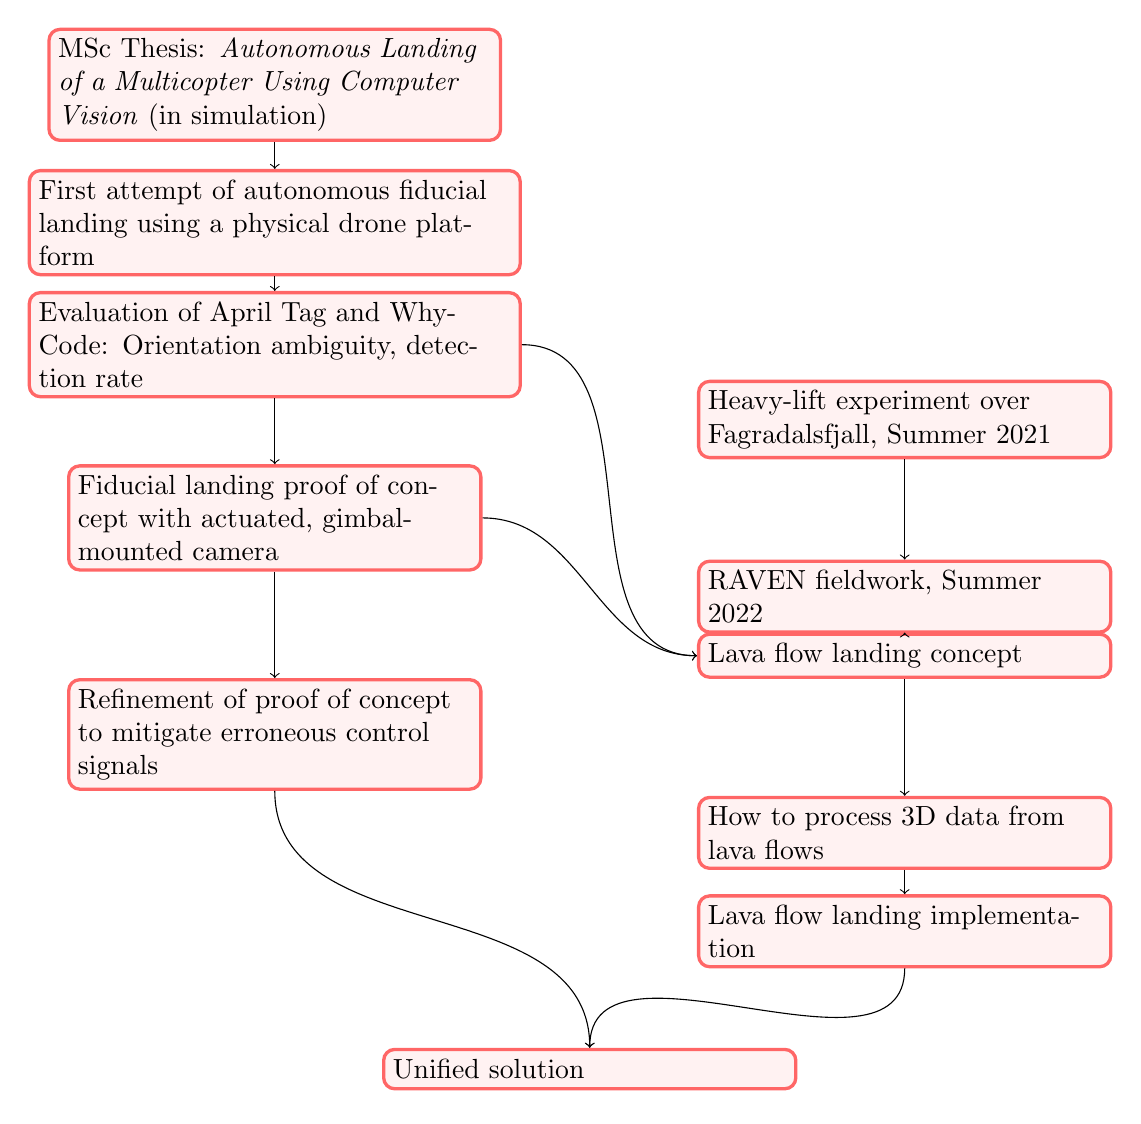
\begin{tikzpicture}[
roundnode/.style={circle, draw=green!60, fill=green!5, very thick, minimum size=7mm},
squarednode/.style={rounded corners, draw=red!60, fill=red!5, very thick, minimum size=5mm},
]
%Nodes
\node[squarednode, text width=5.5cm] (msc) at (0,0) { MSc Thesis: \emph{Autonomous Landing of a Multicopter Using Computer Vision} (in simulation) };
\node[squarednode, text width=6cm] (first_attempt) at (0,-1.75) { First attempt of autonomous fiducial landing using a physical drone platform };
\node[squarednode, text width=5cm] (raven_fagradalsfjall) 	at (8,-4.25) 	{ Heavy-lift experiment over Fagradalsfjall, Summer 2021 };
\node[squarednode, text width=6cm] (evaluation) 		at (0,-3.3) 	{ Evaluation of April Tag and WhyCode: Orientation ambiguity, detection rate};
\node[squarednode, text width=5cm] (poc) 			at (0,-5.5) 	{ Fiducial landing proof of concept with actuated, gimbal-mounted camera };
\node[squarednode, text width=5cm] (raven_fieldwork_2022)	at (8,-6.5)	{ RAVEN fieldwork, Summer 2022 };
\node[squarednode, text width=5cm] (lava_landing_concept)	at (8, -7.25)	{ Lava flow landing concept };
\node[squarednode, text width=5cm] (refinement)			at (0,-8.25)	{ Refinement of proof of concept to mitigate erroneous control\\signals };
\node[squarednode, text width=5cm] (lava_processing)		at (8,-9.5)	{ How to process 3D data from lava flows };
\node[squarednode, text width=5cm] (lava_landing_implementation)		at (8,-10.75)	{ Lava flow landing implementation };
\node[squarednode, text width=5cm] (unified)		at (4,-12.5) 	{ Unified solution };

%Lines
\draw[->] (msc.south) -- (first_attempt.north);
\draw[->] (first_attempt.south) -- (evaluation.north);
\draw[->] (raven_fagradalsfjall.south) -- (raven_fieldwork_2022.north);
\draw[->] (evaluation.south) -- (poc.north);
\draw[->] (poc.south) -- (refinement.north);
\draw[->] (refinement.south) to [out=270,in=90] (unified.north);
\draw[->] (raven_fieldwork_2022.south) -- (lava_landing_concept.north);
\draw[->] (lava_landing_concept.south) -- (lava_processing.north);
\draw[->] (lava_processing.south) -- (lava_landing_implementation.north);
\draw[->] (lava_landing_implementation.south) to [out=270,in=90] (unified.north);
\draw[->] (evaluation) to [out=0,in=180] (lava_landing_concept);
\draw[->] (poc) to [out=0,in=180] (lava_landing_concept);


\end{tikzpicture}
\end{center}
